\documentclass[12pt]{article}
\usepackage{amsmath}
\usepackage{graphicx}
\usepackage{hyperref}
\usepackage[latin1]{inputenc}
\documentclass{article}
\usepackage[utf8]{inputenc}
\usepackage{subfiles}
\title{

\centering

\includegraphics[0.2]{2.png}

\newline
\newline
\centering
\hspace{2cm}\textbf{Capstone Project II}\newline	\newline
		\centering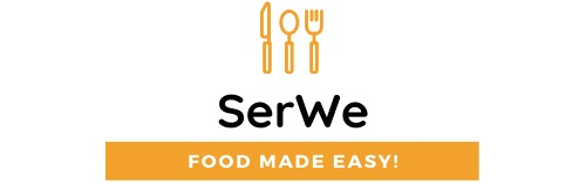
\includegraphics[0.2]{1.png} 

       \textbf{A Online Food ordering App}
\textbf{Milestone 1 - Error 404 Not Found}
\centering
Submitted by
\newline
Rizul Goyal (C0766598)
\newline
Ritik Jagpal (C0762067)
\newline
Anmol Sharma (C0761755)
\newline
Kuldeep Singh Bamrah (C0757769)
\newline
}





\begin{document}
\maketitle
\section{Abstract}
All of the capstone project is often designed in order to show the skills and the abilities learn by the student during the study period. As this capstone project is the part of the Mobile Application Design and Development course in third semester at Lambton College. Kuldeep Bamrah, Rizul Goyal, Anmol Sharma and Ritik Jagpal are working together in a team on Food delivery Application “SerWe”. There are many other similar well-established applications in the market, but we are trying to ignite our own idea to come up with something and challenging to show cast our skills. 

\newline
\section{Introduction}
Everyday new technology is developing with rapid pace we all are the witness and using it in daily life there are multiple things that are become a part of our life. Mobile phones are one of them and we are using it every day and every time. Ordering food is a one of the most popular application uses by people worldwide. The customers of today are not only attracted because placing an order online is very convenient but also because they have visibility into the items offered, price and extremely simplified navigation for the order.\\
The name of our application is “SerWe”. It’s an android application that helps the customer to order the food in easiest way possible. As nowadays everyone is busy, so some find tough to travel to the restaurants to get their food and in order to solve this we have come up with an application that makes a lot easier to order food online.\\
Our group is working on food delivery application “SERWE”. Serwe provides two interfaces for the two types of users i.e. two Android mobile applications one for customers and another for restaurant staff members.
\section{The context of study}
The context of application is the process of ordering food online without having to go to the restaurant. It is a simple and convenient way for customers to purchase food. This is why, Food Ordering App is going to be develop. This project aims to build an application program that would serve as an online platform for ordering food. 

This project also aims to reduce the manual work for managing the food items information, orders of customers, deliveries and payments. SerWe provides two interfaces for the two types of users in restaurants i.e. two Android mobile applications for customers and restaurant staff members.

The Android mobile application allows customers to have a seamless dining experience with features such as Available tables at the restaurant easier, ordering dishes through an interactive menu and being able to pay the bill from their phone.

\section{Motivation}

Food ordering business in trending now days. People prefer to order food online instead of visiting the restaurants to buy a food, so after reviewing the digital or online market we reached at the conclusion that we will continue to develop this food ordering application. Which will generate great revenue in the future.

We personally do not like waiting for long in the restaurants or to have to call restaurants to place an order especially during the peak lunch or dinner hours. Moreover, we value recent learning about the iOS and Android Programming languages as well as seeing how powerful and dynamic they are when it comes to design and create big applications. The languages used to build this application are Android using Java and xml whereas Firebase database at the backend because We found them to be extremely useful while working on the technologies.

\section{Target Audience}

Once you build your marketing strategy for food delivery app the first move is to determine who you are going to target. Tests that show information such as the main demographic and social patterns you can benefit from need to be carried out. You would also need to perform work on your rivals for better results. It can help you determine which groups are more difficult to reach and which future consumers are currently in use. Our main targeted audience are foodie persons who love to order food online on daily basis. 

\section{Market Plans}

Before anything else, you need to ensure that your food app has a solid online presence and got everything needed to acquire high ranking on search engines & to attract more traffic. That’s where search engine marketing comes into the picture as a mix of SEO & PPC ads. Here is what you need to ensure in that regard:

\title{Our team would work to promote our Serwe App on Social Media Platforms such as Instagram, Twitter, Facebook etc. }

\title{Our team would attract the traffic by offering some discounts and coupons}

\title{Showing some video content of app design is another way to attract the people and magnetize your apps.}


\title{Putting up advertisements of app on some related apps is another way of marketing's.}

\section{User Value}

Our food app - serve would serve best user value in the future.By using our online food ordering app, user would get better restaurant services. It would be very easy for the food lovers to order food online with a single click. They would also love the feature of booking table online while going for a dine-in treat.\\ \newline
\section{Work Breakdown Structure}
Breaking work into smaller tasks is a common productivity technique used to make the work more manageable and approachable. For projects, the Work Breakdown Structure (WBS) is the tool that utilizes this technique and is one of the most important project management documents. It singlehandedly integrates scope, cost and schedule baselines ensuring that project plans are in alignment.
\begin{figure}
\centering
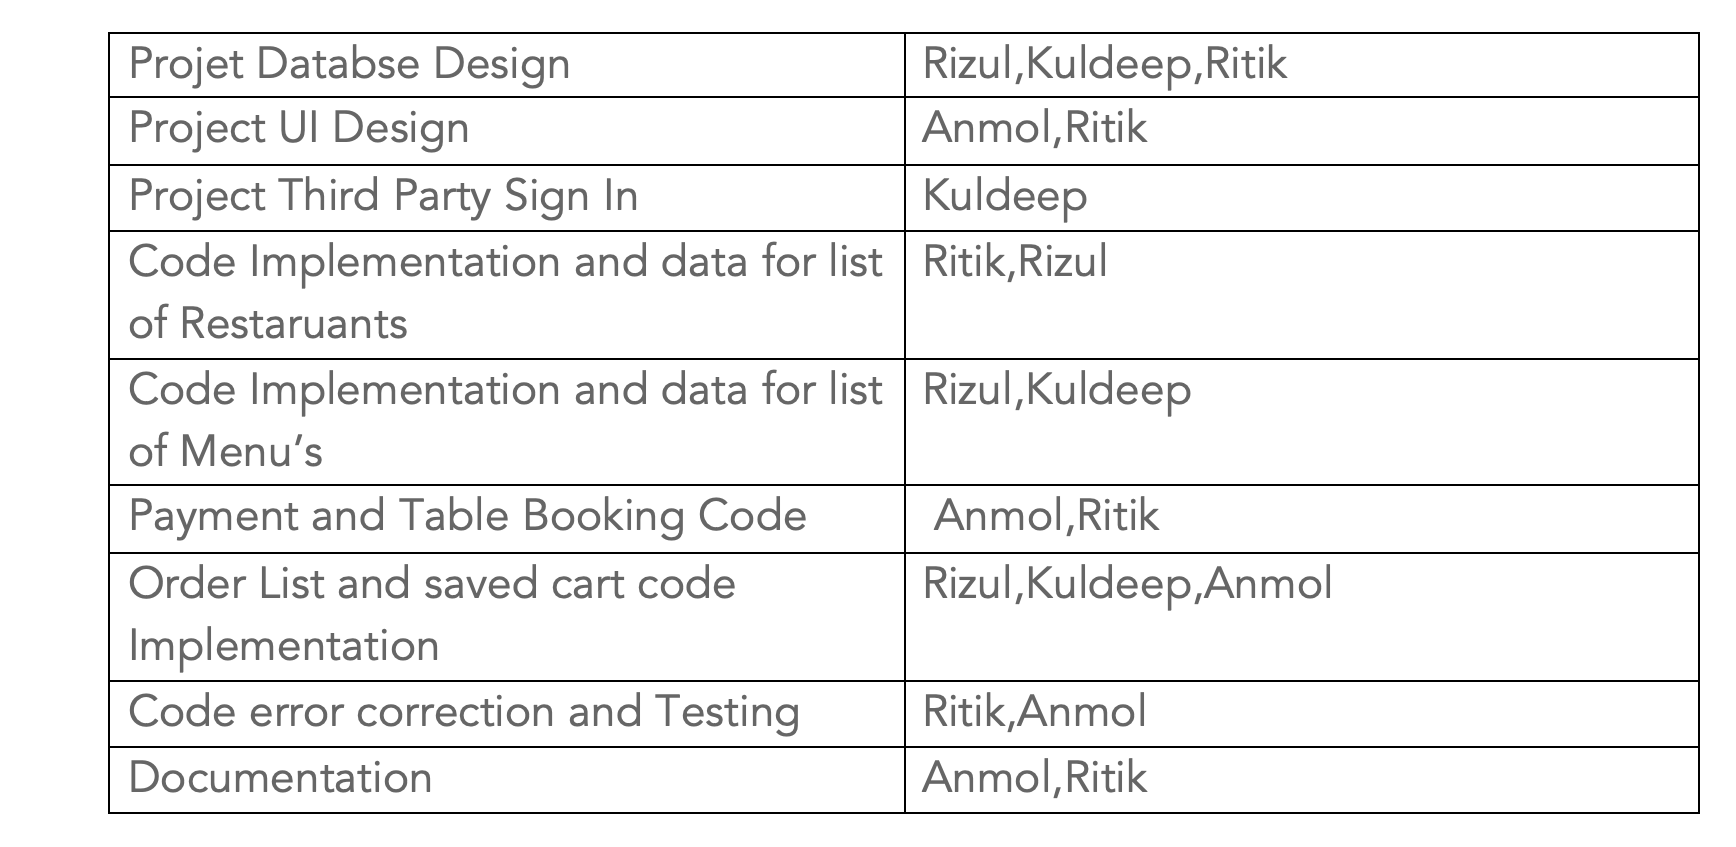
\includegraphics[scale=0.55]{wbspic.png}
\caption{Work Breakdown Structure}
\end{figure}

\section{App monetizing }
Online food delivery apps are a major trend these days as plenty of people simply love to place an order for food from the comfort of their own homes.\\
Food delivery in Canada has transitioned from dialing a number, to ordering online to opening an app on your phone. While players have come and gone over the years, these days the industry has mostly consolidated with a handful of big players left.\\



\textbf{The Revenue Model – How The Food Delivery App Makes Money?}\\
There are many ways in which you can monetize your on-demand food delivery mobile application. A few but most commonly applied monetization methods are:\\
\textbf{
1.Delivery Charges}
Many restaurants do not provide home delivery. So when you offer them your on-demand delivery app with food delivery personnel, then the restaurant will most likely pay you delivery charges.The Delivery app made a profit of 164 dollar million last year with this particular revenue model.

 
\\
\textbf{2.Surge Pricing}
Uber Eats implicates a surge price when the demand is too high. In this process, the app limits the menu options and adds a surcharge (peak price) when the customer is placing the order. The rate of demand can be lower, but the per delivery amount can rise to a great extent in this type of revenue model.
 

\textbf{3.Commission}
The food delivery app owner can charge a commission for every order that the customer makes through the app. For generating revenue, companies prefer this revenue model.

This model not only helps in generating high revenues but also helps in creating a long-term relationship between the food delivery app company and the restaurant.

\section{Competitive analysis}

Online food delivery apps are a major trend these days as plenty of people simply love to place an order for food from the comfort of their own homes.

Food delivery in Canada has transitioned from dialing a number, to ordering online to opening an app on your phone. While players have come and gone over the years, these days the industry has mostly consolidated with a handful of big players left.

It can be hard to muster up the strength to leave your home, or the couch, when the temperature drops lower than your motivation to cook. Luckily, there are food delivery apps that add a whole other meaning to comfort food.
\textbf{Uber Eats
}
An American online food ordering and delivery platform launched by Uber in 2014 and based in San Francisco, California
\begin{itemize}
\item Uber Eats is a food delivery platform that makes getting great food from your favorite local restaurants as easy as requesting a ride.The Uber Eats app connects you with a broad range of local restaurants and food, so you can order from the full menus of your local favorites whenever you want.
\end{itemize}
\begin{itemize}
\item Besides, the food delivery application provides users with many functions, making food ordering even more convenient. The most notable food delivery app features are:			
\end{itemize}
			1.Tailored restaurant recommendations\\
			2.Advanced search filters\\
			3.Order tracking\\
			4.Customize delivery details


\textbf{Skip The Dishes
}\\
\\
SkipTheDishes' technology allows customers to order food online. Customers order through the SkipTheDishes website or mobile iOS and Android apps. They can pay for their orders online with credit cards, debit cards, or in-person with cash when their orders arrive. Restaurants receive orders on their integrated mobile apps, and couriers are allocated to orders through their integrated mobile apps. Customers can view the status of their orders through live updates on the app, and are given transparency into the location of their assigned courier through GPS tracking.
\\
Restaurants and couriers can be reviewed by customers after they have received their orders. This helps to provide both feedback and transparency to the rest of the network about the efficiency and effectiveness of its stakeholders.
\\
SkipTheDishes operates across Canada and in select markets in the United States. Since its founding in 2012, SkipTheDishes continues to advance the technological innovation required for building the future of food delivery, while being instrumental in helping to create a tech hub in the Canadian Prairies.
\begin{itemize}
\item It is one of the best food delivery apps in Canada serving the cities of Toronto, Vancouver, Winnipeg, Ottawa among others. According to Crunchbase, It has received a total funding of $2.1B. The company is currently worth more than $13 billion and is the largest third-party delivery service in the world, surpassing Grubhub in 2019. 

\end{itemize}


\textbf{Door Dash}

DoorDash is San Francisco-based on-demand app to deliver food. It was launched in 2013 in San Francisco, California, United States. They now have over 6900 employees and delivery executives that make food delivery as breezy as possible. It has collaborated with over 340,000 selection of stores across the US and Canada.
\begin{itemize}
\item It is one of the best food delivery apps in Canada serving the cities of Toronto, Vancouver, Winnipeg, Ottawa among others. According to Crunch base, It has received a total funding of 2.1B Dollar. The company is currently worth more than 13 billion Dollar and is the largest third-party delivery service in the world, surpassing Grub hub in 2019.
\begin{itemize}
\item Features
\item Search the best restaurants in the town
\item Choose your favourite dishes
\item Pick-up or get it delivered
\item Schedule your order
\item Navigation and directions

\end{itemize}


\end{itemize}


\section{Use Cases}
A use case is a description of a specific interaction between an actor (an entity external to the system, such as a user or another system) and the system being designed.

Use cases add value because they help explain how the system should behave and in the process, they also help brainstorm what could go wrong.  They provide a list of goals and this list can be used to establish the cost and complexity of the system.
Represents the goal of an interaction between an actor and the system. The goal represents a meaningful and measurable objective for the \textbf{actor}. Records a set of paths (scenarios) that traverse an actor from a trigger \textbf{event} (start of the use case) to the \textbf{goal} (success scenarios).


\begin{figure}
\centering
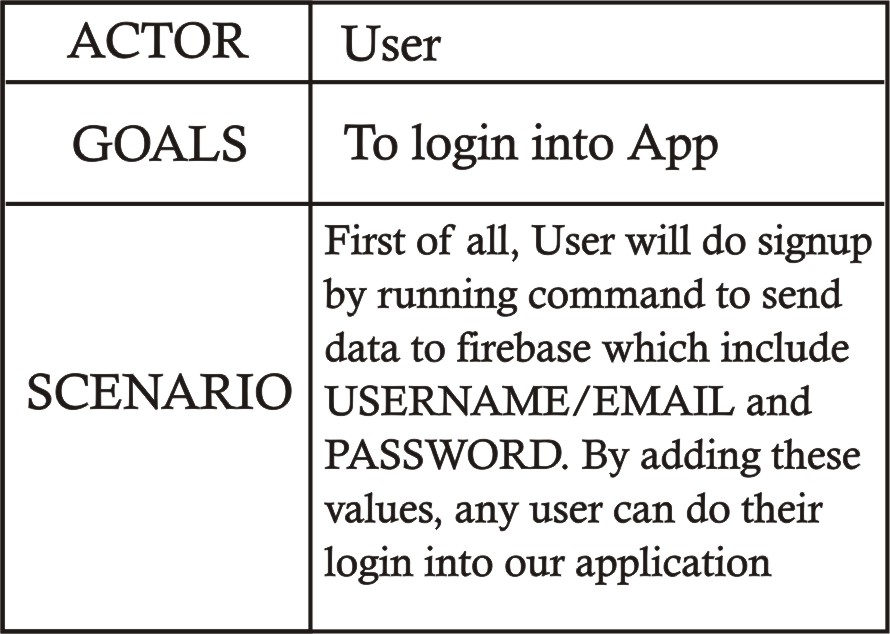
\includegraphics[scale=0.4]{login.jpeg}
\caption{Login}
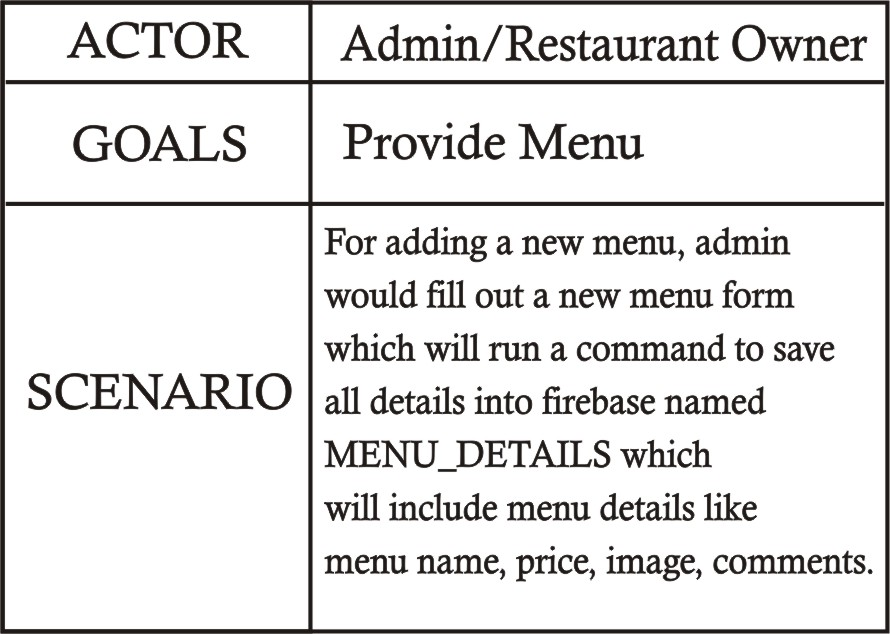
\includegraphics[scale=0.4]{menue.jpeg}
\caption{Menu}
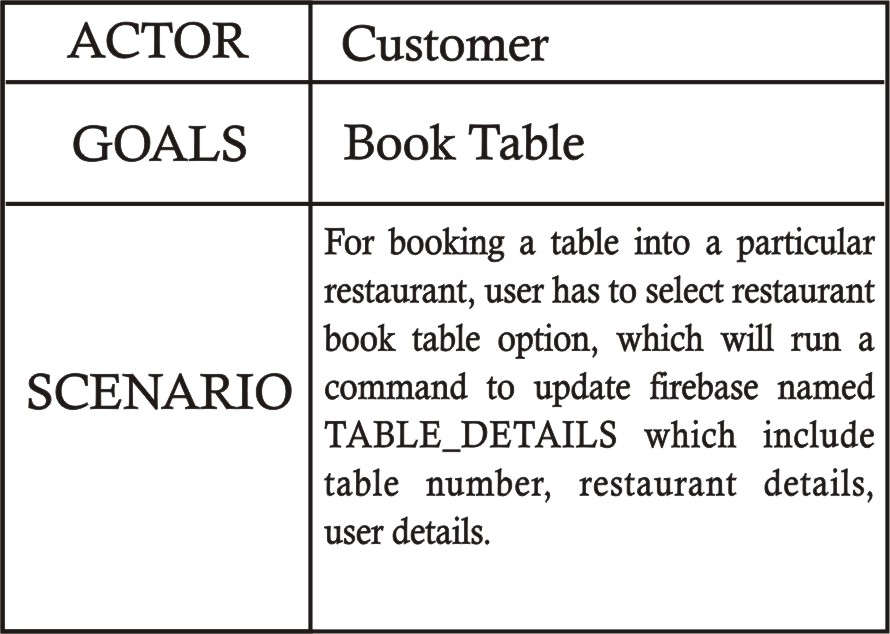
\includegraphics[scale=0.4]{booktabel.jpeg}
\caption{Book table}
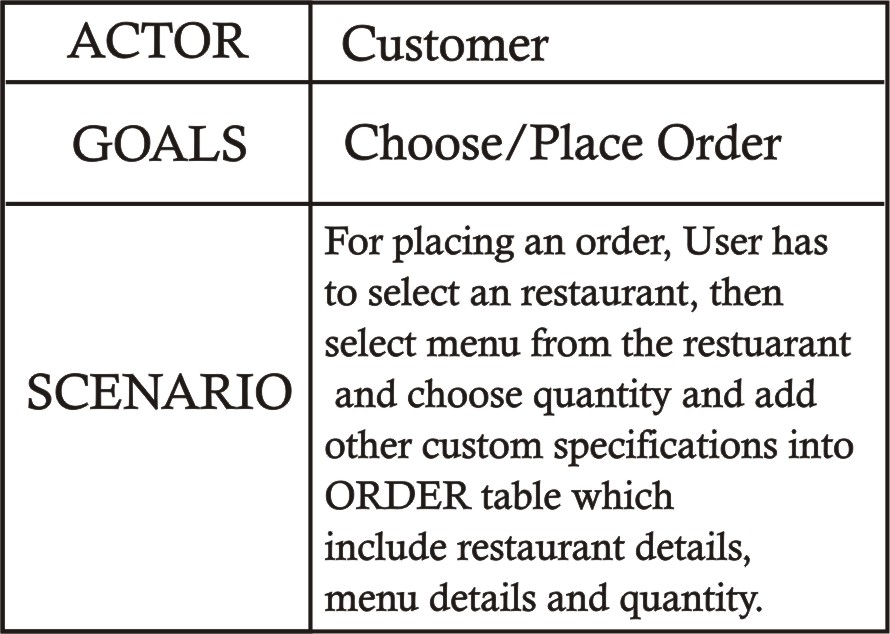
\includegraphics[scale=0.4]{choose.jpeg}
\caption{Choose food}
\end{figure}
\begin{figure}
\centering
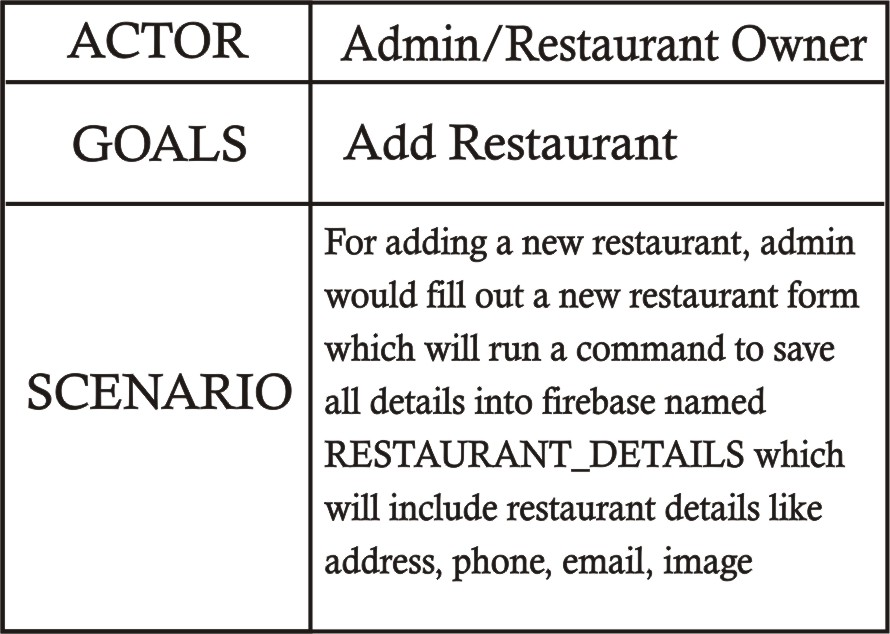
\includegraphics[scale=0.4]{admin.jpeg}
\caption{Admin}
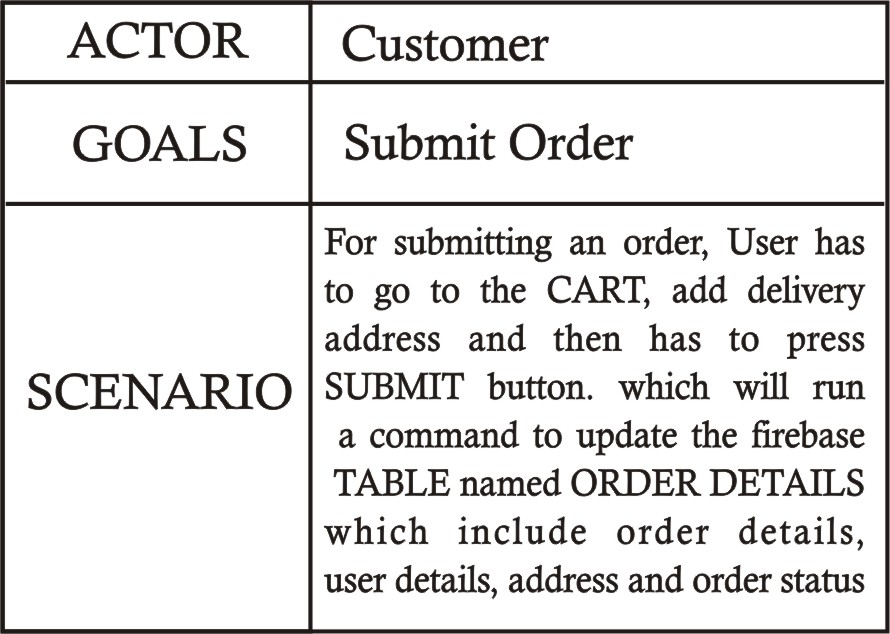
\includegraphics[scale=0.4]{submit.jpeg}
\caption{Submit order}

\end{figure}


\begin{figure}
\centering
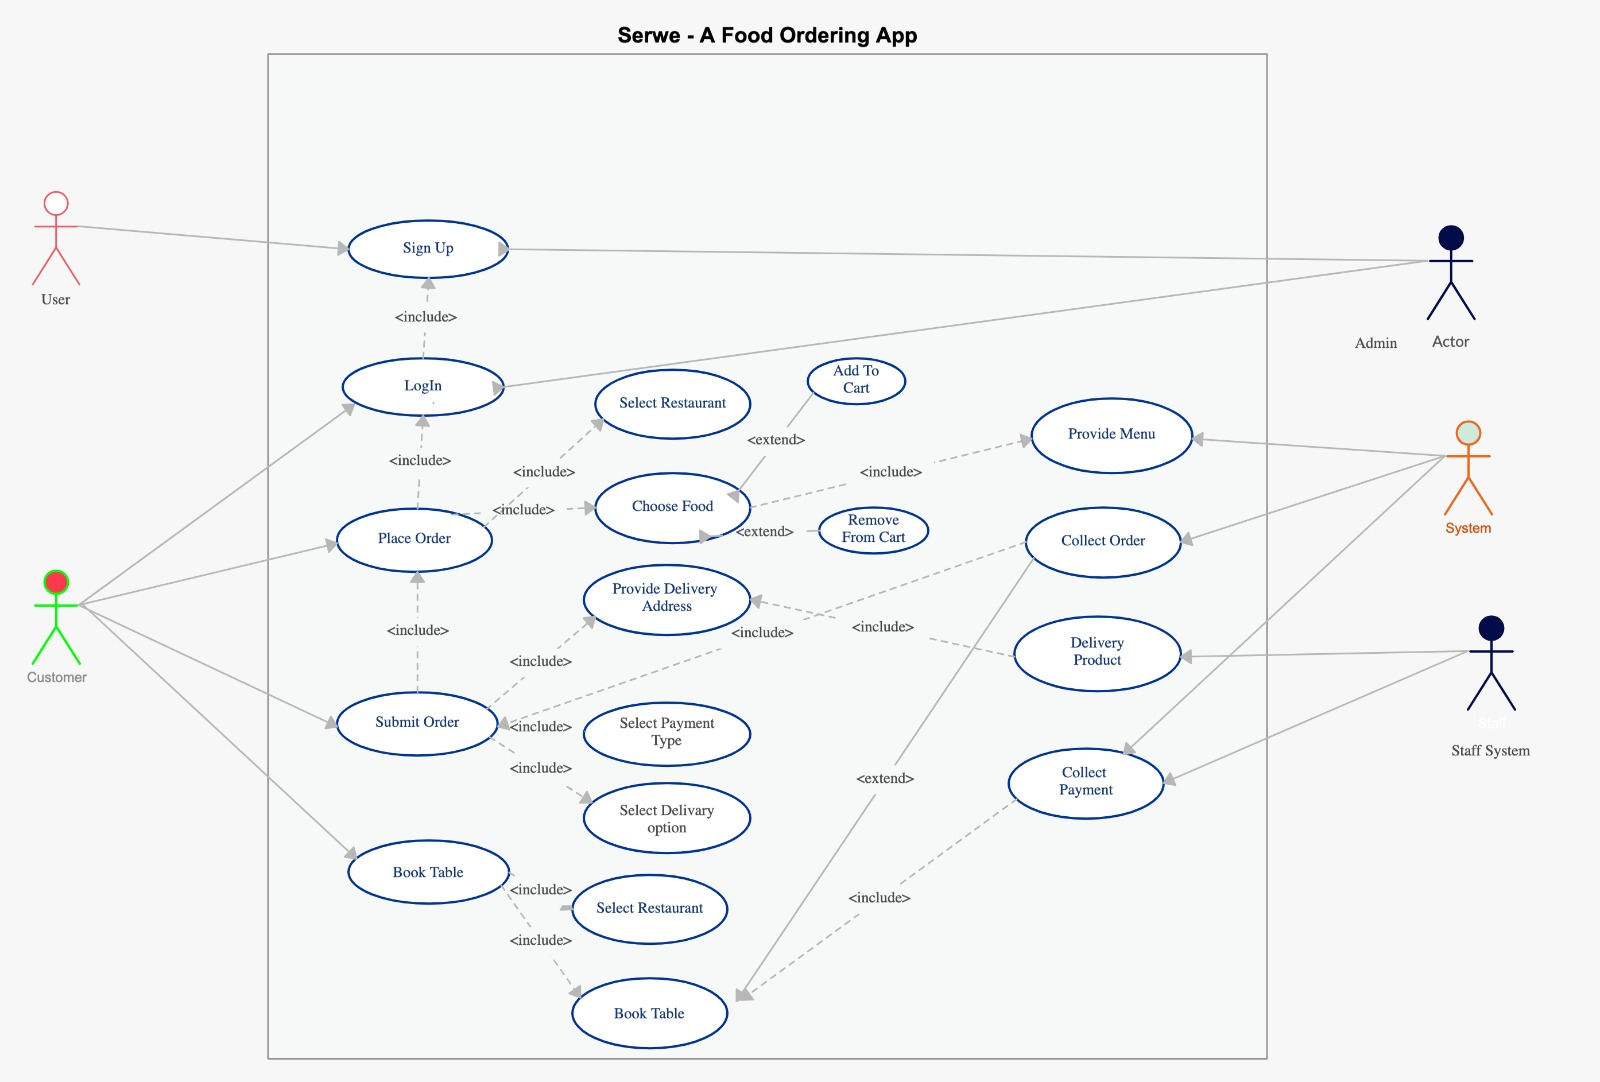
\includegraphics[scale=0.3]{WhatsApp Image 2020-08-17 at 9.15.41 PM.jpeg}
\caption{Use cases}
\end{figure}

\section{Cost Estimation}
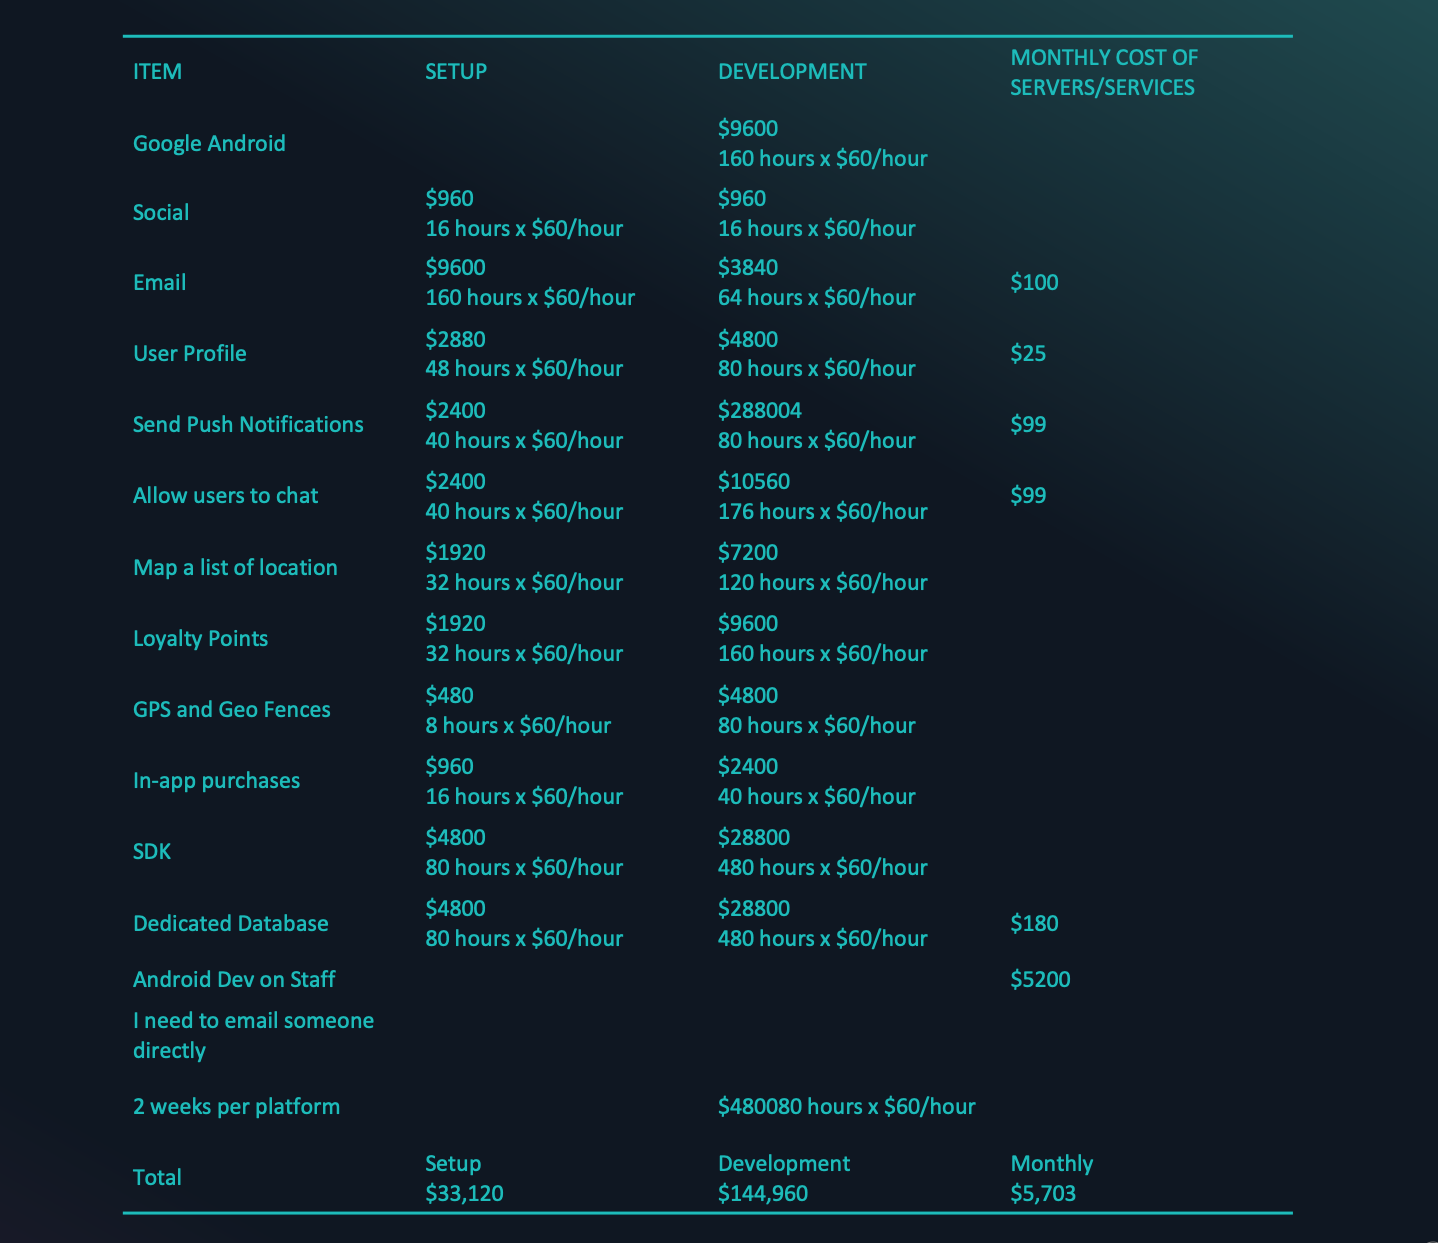
\includegraphics[scale=0.5]{cost.png}




\subfile{milestone2/userstories}

\subfile{milestone2/matrix}


\subfile{milestone2/testcases}
\subfile{milestone2/diagrams}


\section{References}
1.http://www.cs.uno.edu/~jaime/Courses/4210/useCaseFundamentals.html#:~:text=Represents%20the%20goal%20of%20an,the%20goal%20(success%20scenarios).
\newline
2.https://moodle.cestarcollege.com/moodle/my/ \\
3.https://www.similarweb.com/apps/top/google/store-rank/ca/food-and-drink/top-free/ \\
4.https://www.wikipedia.org/ \\
5.https://www.youtube.com/ \\

\end{document}












